\documentclass{bcc}

\titulo{OrCA IDE: Uma IDE geradora de Ontologias}
\palavrasChave{Ontologia}{Linguagem Natural}{OWL}
\keywords{Ontology, Natural Language, OWL}

\autor{Paulo Mateus da Silva}{paulomatew@gmail.com}

\orientador{Ryan Azevedo}{UAG}{UFRPE}
%\orientadorDois{John von Neumann}{UAG}{UFRPE}
% \orientadorTres*{Ada Lovelace}{UAG}{UFRPE} % Se feminino use *, tanto para orientador ou examinador

\examinador{John Hopcroft}{UAG}{UFRPE}
\examinadorDois{Richard Karp}{UAG}{UFRPE}
\examinadorTres{Stephen Cook}{UAG}{UFRPE}
\examinadorQuatro{John Backus}{UAG}{UFRPE}

\dataMesAno{7}{agosto}{2018}

\begin{document}

\selectlanguage{portuguese}

\capa

% \capaDois

\begin{resumo}
INSERIR RESUMO
\end{resumo}

\selectlanguage{english}
\begin{abstract}
INSERIR ABSTRACT
\end{abstract}
\selectlanguage{portuguese}

% Centralizar titulos
\renewcommand\contentsname{\centerline{Sumário}}
\renewcommand\listfigurename{\centerline{Lista de Figuras}}
\renewcommand\listtablename{\centerline{Lista de Tabelas}}

\lhead{Sumário}
\tableofcontents

\listoffigures
\addcontentsline{toc}{chapter}{Lista de Figuras}

\listoftables
\addcontentsline{toc}{chapter}{Lista de Tabelas}

\inicio
\chapter{Introdução}

TEXTO


\section {Contextualização}

TEXTO

\section{Motivação e Justificativa}

TEXTO


\section{Definição do Problema}

TEXTO

\section{Objetivo}

TEXTO

\section{Organização do Relatório}

Além deste capítulo inicial que traz uma introdução sobre o tema, a motivação e justificativa para realização do trabalho, a definição do problema e o objetivo; este trabalho está organizado em mais X capítulos, como seguem:

• O \autoref{chap:fundamentacao} apresenta a fundamentação teórica, contendo referências bibliográficas de estudos na área e apresenta as ferramentas e conceitos que foram utilizados no desenvolvimento;

• O \autoref{chap:atividades}

• O \autoref{chap:sistema} mostra a arquitetura do sistema e a maneira que ele foi construído, utilizando os conceitos e ferramentas que foram previamente apresentados no capítulo \autoref{chap:fundamentacao}.

• O \autoref{chap:atividades} expõe os experimentos que foram realizados e seus respectivos resultados, exibindo assim, o funcionamento do sistema.


\chapter{Fundamentação teórica}
\label{chap:fundamentacao}

Nesta seção são apresentados os conceitos e ferramentas que foram utilizados no desenvolvimento deste projeto e as respectivas justificativas que embasam o uso de cada um deles.

\section{Ontologia}

Existem diversas técnicas que podem ser utilizadas para organizar informações e conhecimento, a aplicação de ontologias tem recebido uma atenção cada vez maior \cite{almeida2014}. O termo pode ser encontrado não apenas na ciência da computação, mas também em diversas áreas do conhecimento, por isso, é importante entender seu significado e sua aplicação em cada área específica.

\subsection{Histórico e Definições}

A palavra ontologia está presente em diversas áreas do conhecimento e possui diferentes significados para cada uma delas. Devido ao seu
uso diversificado, seu significado tende a ser muito vago. Dessa forma, existem muitas definições para o termo \cite{gava2003}.

O termo ontologia teve origem no século XVII na área da filosofia, a palavra vem do grego e pode ser traduzida como estudo da existência \cite{guizzardi2005}. Segundo \cite{gruber1995} o termo é emprestado da filosofia onde uma Ontologia é uma explicação sistemática da existência. Para um sistema de Inteligência Artificial, o que existe é tudo aquilo que pode ser representado.

Na computação, o termo foi usado pela primeira vez no fim dos anos 70 e desde então, ontologias têm sido aplicadas em uma infinidade de áreas da ciência da computação, uma das motivações foi a necessidade de criar representações de princípios de conhecimento de domínio na comunidade de compartilhamento e reutilização de conhecimento em IA \cite{guizzardi2005}.

Em áreas relacionadas com Modelagem Conceitual, ontologias são usadas de acordo com dua definição em Filosofia. Na Inteligência Artificial, Engenharia de Software e \textit{Web} Semântica geralmente ontologia é usada como: (i)um artefato concreto de engenharia desenhado com um intuito específico sem focar muito em questões de fundamentação ou (ii) uma representação de um domínio particular que pode ser expressa em alguma linguagem de representação de conhecimento (RDF, OWL, F-Logic) ou de modelagem conceitual (UML, EER) \cite{guizzardi2008}. Neste trabalho, será considerada a definição ii, que é a mais utilizada na área de Inteligência Artificial.

Segundo \cite{gruber1995} uma ontologia é uma especificação explícita de uma conceituação. \cite{lv2011} afirma que o principal papel das ontologias é melhorar a comunicação entre humanos ou entre computadores, especificando a semântica do aparato simbólico usado no processo de comunicação.

\section{OWL}

A \textit{Web Ontology Language} (OWL) é projetada para ser usada por aplicações que precisam processar o conteúdo da informação em vez de apenas apresentar informações aos seres humanos. OWL fornece uma maior facilidade para a máquina interpretar o conteúdo da Web do que linguagens suportadas por XML, RDF e RDF Schema (RDF-S), pois fornece vocabulário adicional junto com uma semântica formal. Ela possui três sub-linguagens cada vez mais expressivas: OWL Lite, OWL DL e OWL Full \cite{mcguinness}.

\subsection{OWL Manchester Syntax}

TEXTO d hsdgsdfghdfghdfghdfghdfghdfghdfghdfgh

\section{Pellet}

Pellet é implementado em Java e é \textit{open source}, ele fornece uma gama de recursos como: suporte a regras, conexão de raciocínio, identificação de axiomas. Para tornar seus recursos de raciocínio acessível aos usuários, ele fornece diferentes interfaces \cite{sirin2007}.

Os recursos do Pellet são expostos a partir de uma API Java, uma interface de linha de comando ou um formulário da Web. Ele fornece acesso programático às funções de raciocínio por meio de duas interfaces diferentes, uma para o kit de ferramentas do Jena e uma para a biblioteca da API do OWL \cite{parsia2004}. No desenvolvimento da ferramenta em questão o Pellet foi utilizado a partir de uma API Java e suas funções foram acessadas através da biblioteca do OWL.

\section{Arquitetura MVC}

MVC (\textit{Model View Controller}) é um padrão de arquitetura de \textit{software} que sugere uma divisão de componentes, permitindo assim, um código mais organizado e simples além de facilitar e tornar mais segura a manutenção do sistema \cite{da2012}. Essa arquitetura se tornou popular no desenvolvimento de sistemas complexos, pois, ela auxilia na separação dos principais componentes do sistema, além de apoiar a manipulação, gerenciamento e armazenamento dos dados \cite{de2013}.

Nessa abordagem, em resumo, o sistema é dividido em três componentes interconectados: \textit{model}, que expressa o conhecimento do domínio, \textit{view}, que apresenta a interface do usuário e \textit{control} que gerencia as atualizações para as \textit{views} \cite{selfa2006}.
 
 \textit{Model} é a camada responsável pela manipulação e gerenciamento dos dados, ou seja, faz a leitura, escrita e validação dos dados, e se houver necessidade, também permite a comunicação do banco de dados. Ela contém os dados do aplicativo, a definição lógica, a especificação da função e o envolvimento da regra de negócios. O \textit{model} pode ser um único objeto ou uma composição de objetos \cite{jailia2016}.
 
 \textit{View} é a camada de interação com o usuário, é responsável por exibir todos os dados do contidos no \textit{model}. Mostra apenas os atributos necessários e oculta os atributos desnecessários, fornecendo assim uma apresentação encapsulada \cite{jailia2016}.
 
 Por fim, \textit{controller} é a camada que recebe todas as requisições do usuário e faz a sua conexão com o sistema. Ele controla o \textit{model} a ser utilizado assim como seu fluxo de dados, e atualiza a exibição na \textit{view} que será mostrada ao usuário \cite{jailia2016}. 

\section{Java}

TEXTO

\section{Maven}

O Maven é uma ferramenta de integração de projetos Java utilizada no gerenciamento e automação de construção (build) de projetos, além disso, fornece diversas funcionalidades adicionais através do uso de \textit{plugins} e estimula o emprego de melhores práticas de programação \cite{maven}.

A ferramenta surgiu da dificuldades que muitos grupos de desenvolvimento tinham ao gerenciar bibliotecas em grandes projetos, de maneira dinâmica o Maven baixa a biblioteca Java e os seus \textit{plugins} de diversos repositórios que ficam armazenados em cache local, que pode ser atualizado quando sempre que for preciso \cite{oliveira2016}. Sua configuração é feita através do arquivo pom.xml (Project Object Model) onde são declarados o tipo de empacotamento, suas dependências e os repositórios de onde as dependências serão buscadas, podendo ser tanto repositórios locais ou remotos. \cite{junior2014}


\section{Compilador}
TEXTO (Analisadores, lexema, lookahead, regra de produção, gramática)

De maneira geral, um compilador é um programa que tem como entrada um código de programa numa certa linguagem e produz como saída um código de programa numa outra linguagem, preservando o significado do código durante esse processo \cite{grune2012}.

Um compilador é dividido em fases, cada uma delas representam uma etapa do processo de compilação, elas podem ser desenvolvida de maneira separada, mesmo que na prática elas funcionem intercaladamente \cite{foleiss2009}.

\subsection{Analisador Léxico}

\subsection{Analisador Sintático}

\subsection{Analisador Semântico}

\chapter{Atividades Desenvolvidas}
\label{chap:atividades}

TEXTO

\chapter{Arquitetura do Sistema}
\label{chap:sistema}

\section{Introdução}
Com a finalidade de criar uma ontologia a partir de  Processamento de Linguagem Natural (PLN), o sistema OrCA IDE (\textit{Ontology vieweR and CreAtor Integrated Development Environment}) foi desenvolvido. Neste capítulo são detalhadas a arquitetura do sistema e suas funcionalidades, bem com a linguagem natural controlada utilizada. O intuito, ao definir esta linguagem, foi facilitar ao máximo o desenvolvimento das ontologias por parte dos usuários do sistema.

\section{Arquitetura}

O sistema foi implementado utilizando a arquitetura **********, visando otimizar o desenvolvimento e facilitar a manutenção do código fonte. Qualquer programador que visualizar a estrutura do projeto e desejar realizar ajustes, não terá dificuldade em achar seus componentes. Na Figura \ref{fig:pacotesJava} é possível visualizar todos os pacotes do projeto.

\begin{figure}[H]
\centering
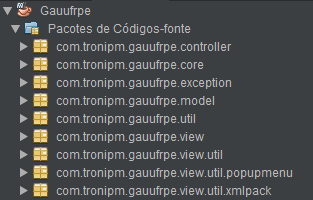
\includegraphics[width=.6\textwidth]{Figuras/estrutura.png}
\caption{Pacotes de classes no projeto}
\label{fig:pacotesJava}
\end{figure}

\section{Componentes}
O sistema possui 4 componentes (telas): \textit{Compiler}, \textit{Ontology}, \textit{Reasoner} e \textit{Graph Viewer}. Detalhes de cada componente do sistema serão vistos nas subseções seguintes. Todos os componentes que serão descritos a seguir podem ser localizados no pacote exibido na Figura \ref{fig:pacotesView}. 

\begin{figure}[H]
\centering
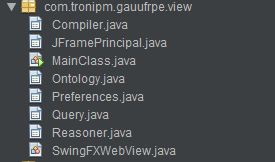
\includegraphics[width=.6\textwidth]{Figuras/pacote_view.png}
\caption{Pacote contendo os principais componentes.}
\label{fig:pacotesView}
\end{figure}

\subsection{Compiler}

O \textit{compiler} é responsável por receber a linguagem natural do usuário e retornar se essa linguagem natural pode ou não ser compilada, assim como mostrar eventuais erros que impossibilitam a compilação. A Tela completa pode ser vista na Figura \ref{fig:telaCompiler}.


\begin{figure}[H]
\centering
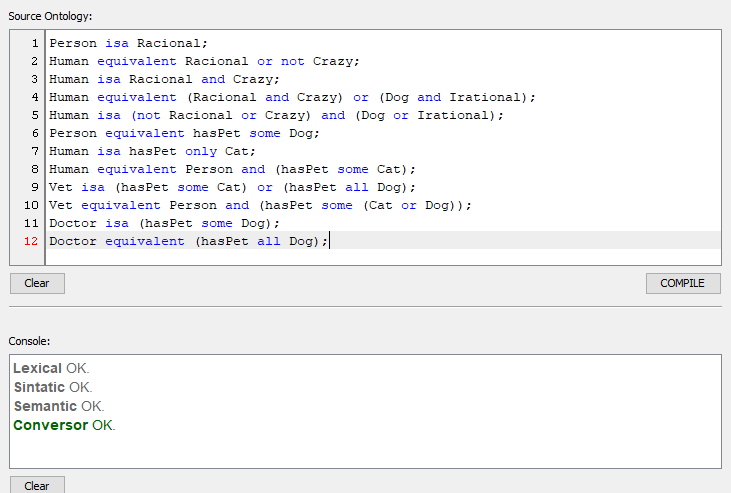
\includegraphics[width=.7\textwidth]{Figuras/tela_compiler.png}
\caption{Tela \textit{Compiler} completa}
\label{fig:telaCompiler}
\end{figure}

Como podemos ver na Figura \ref{fig:telaCompiler1}, o campo de texto chamado \textit{Source Ontology} é onde o usuário irá inserir a linguagem natural. O botão \textit{Clear} tem a função de apagar todo o conteúdo desse campo de texto, e o botão \textit{COMPILE} faz a compilação da linguagem utilizada pelo usuário. 

\begin{figure}[H]
\centering
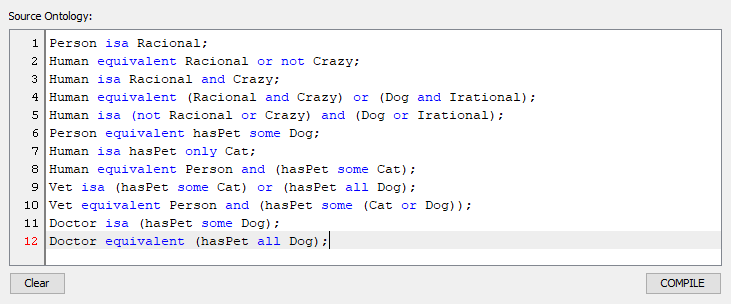
\includegraphics[width=.7\textwidth]{Figuras/tela_compiler1.png}
\caption{Tela \textit{Compiler}: parte da edição da Linguagem Natural}
\label{fig:telaCompiler1}
\end{figure}

Na mesma tela, porém no campo Console, é possível ver a saída do compilador com uma mensagem amigável para o usuário, como visto na Figura \ref{fig:telaCompiler2}. Há 5 tipos de saídas no console: 

\begin{enumerate}
  \item \textbf{Lexical OK}: passou sem erros pelo analisador léxico;
  \item \textbf{Sintatic OK}: passou sem erros pelo analisador sintático;
  \item \textbf{Semantic OK}: passou sem erros pelo analisador semântico;
  \item \textbf{Conversor OK}: a linguagem utilizada pelo usuário foi convertida com sucesso para uma ontologia.
  \item \textbf{Erros}: ao passo que algum erro seja encontrado, o console (Figura \ref{fig:telaCompiler2}) irá mostrar em qual linha, coluna e palavra aconteceu o erro.
\end{enumerate}

\begin{figure}[H]
\centering
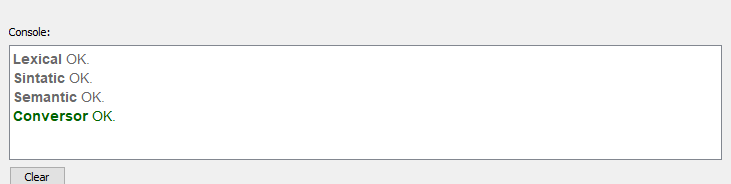
\includegraphics[width=.7\textwidth]{Figuras/tela_compiler2.png}
\caption{Tela \textit{Compiler}: retorno da compilação da linguagem natural}
\label{fig:telaCompiler2}
\end{figure}

\subsection{Ontology}

A \textit{Ontology} mostra a saída da ontologia (em OWL) após a compilação da linguagem natural do usuário. Este campo não é editável, porém, embora o usuário não possa inserir ou remover texto, o modelo de visualização pode ser alterado através do menu suspenso chamado \textit{Output Model} para as seguintes sintaxes: \textit{RDF/XML} (padrão), \textit{KRSS2, Latex, Manchester OWL Syntax, OWL/XML, OWL Functional Syntax} e \textit{Turtle}. Todas essas sintaxes são fornecidas pela \textit{Manchester OWL API}. 

O botão \textit{Graph} tem a função de abrir o componente \textit{Graph}, e o botão \textit{Copy} a de enviar o texto que está aparecendo no campo de texto para a área de transferência. Na Figura \ref{fig:telaOntology} é possível observar a Tela \textit{Ontology} completa.

\begin{figure}[H]
\centering
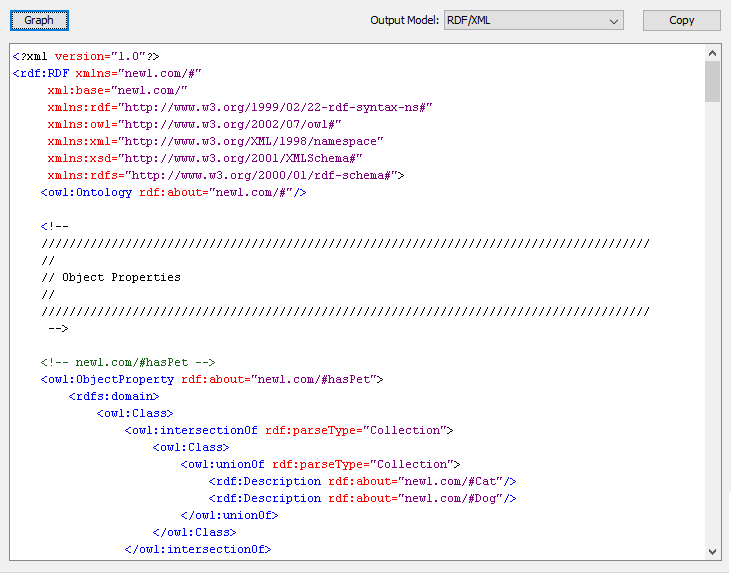
\includegraphics[width=.7\textwidth]{Figuras/tela_ontology.png}
\caption{Tela Ontology}
\label{fig:telaOntology}
\end{figure}

\subsection{Reasoner}

Se tratando de ontologias, um \textit{reasoner} é um software capaz de inferir consequências lógicas sobre a ontologia, muitas vezes não explícitas na sua base de conhecimento. O campo de texto superior do componente \textit{Reasoner} é onde é mostrada a saída que o \textit{reasoner} integrado ao sistema (\textit{Pellet}) conseguiu deduzir através da ontologia inserida (linguagem natural). No início da saída, ele informa se na ontologia base (a linguagem natural inserida pelo usuário) existe algum tipo de inconsistência, por exemplo: "Gato não é vaca (Gato is not Vaca)" e mais a frente existir o axioma "Gato é vaca (Gato is Vaca)", isso vai gerar um aviso de inconsistência, porém, a dedução de novos axiomas ainda será realizada.

O botão \textit{Reason} refaz o processamento de deduzir sobre a ontologia base. O campo de texto \textit{Ontology Inferred} é o código \textit{OWL} da nova ontologia criada a partir dos axiomas deduzidos. O botão \textit{Save on Text File} tem a função de abrir uma caixa de diálogo permitindo que o usuário salve essa nova ontologia em seu computador. A Figura \ref{fig:telaReasoner} mostra essa tela completa.

\begin{figure}[H]
\centering
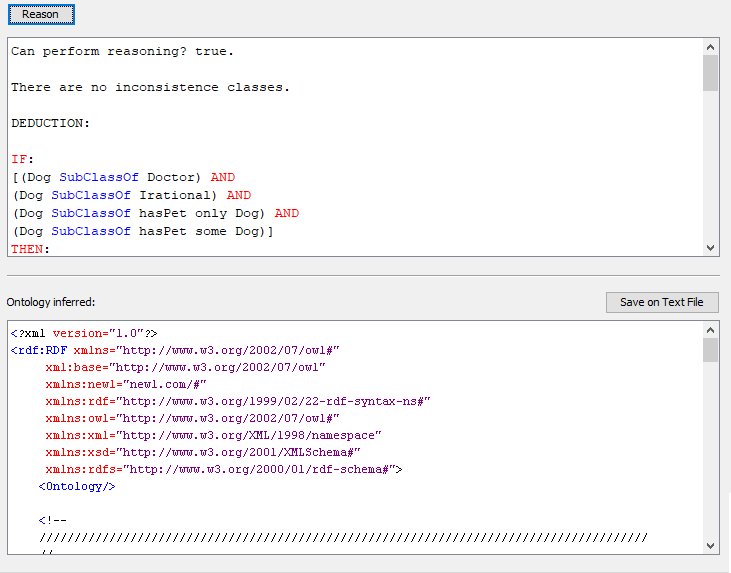
\includegraphics[width=.7\textwidth]{Figuras/tela_reasoner.png}
\caption{Tela Reasoner}
\label{fig:telaReasoner}
\end{figure}

\subsection{Graph Viewer}

\textit{Graph Viewer} é apenas um facilitador gráfico, afim de mostrar a ontologia compilada em forma de grafo. A Figura \ref{fig:telGraph} mostra a tela \textit{Graph Viewer}, que é responsável por mostrar ao usuário uma perspectiva de grafo da ontologia criada. Nela é possível aumentar e diminuir zoom, assim como exportar tanto em arquivo de imagem no formato SVG como em texto no formato JSON. É possível também movimentar os nós, bem como aumentar ou diminuir o tamanho desses, para facilitar a visualização.

\begin{figure}[H]
\centering
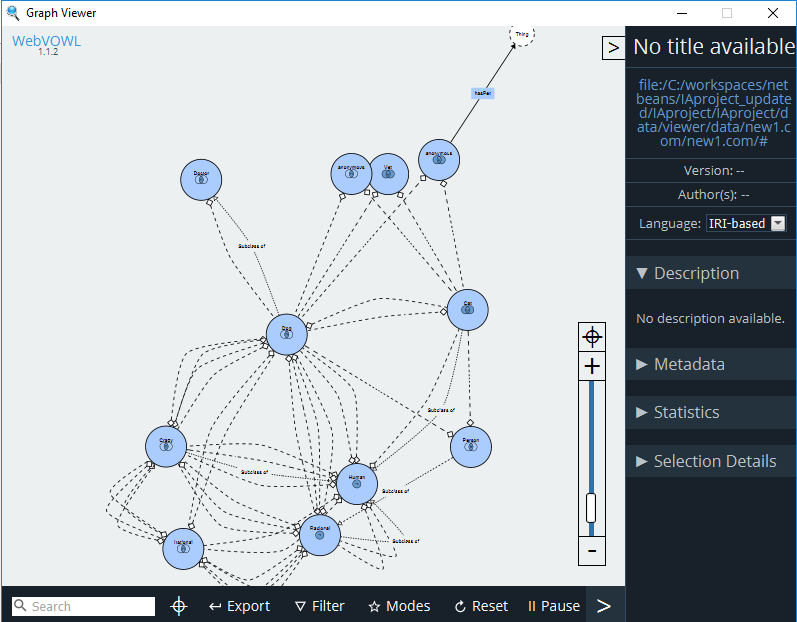
\includegraphics[width=.7\textwidth]{Figuras/tela_graph.png}
\caption{Tela Graph Viewer}
\label{fig:telGraph}
\end{figure}

\section{Compilador}

Um compilador é um tipo de programa que traduz um código descrito em alto nível, ou seja, mais legível e fácil de entender pelo ser humano, em um código semanticamente equivalente em baixo nível, não legível pelo ser humano e não necessariamente executável pela máquina. Geralmente um compilador não traduz imediatamente um código de máquina, mas sim um código intermediário, em linguagem simbólica, só a partir deste momento o código é traduzido para uma linguagem de máquina. De forma semelhante, o compilador desenvolvido para a OrCA IDE não irá traduzir o código descrito pelo usuário para um código de máquina, mas sim para um código "intermediário", o \textit{OWL 2 DL}, que para os fins desse projeto já é o código final.

Para um programa ser definido como um compilador, ele precisa ter alguns processos, são eles: análise léxica, análise sintática, análise semântica e conversor. Juntos, esses quatro processos formam  o ciclo necessário para um compilador verificar se o código descrito pelo usuário não possui erros e pode ser compilado. O fluxo de um compilador padrão pode ser observado na Figura \ref{fig:compilerscheme}.

\begin{figure}[H]
\centering
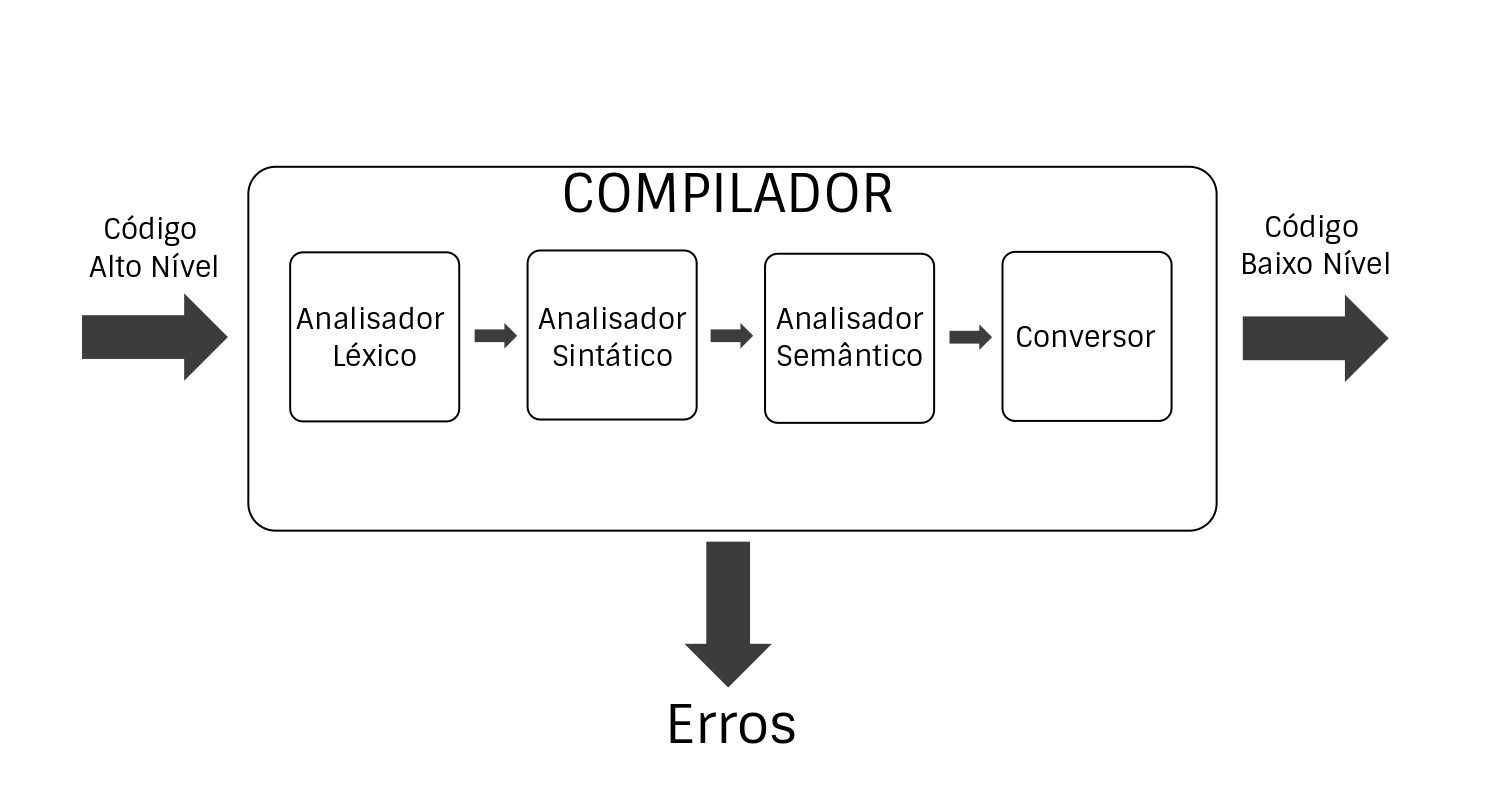
\includegraphics[width=.7\textwidth]{Figuras/compiladorscheme.png}
\caption{Fluxo de um compilador}
\label{fig:compilerscheme}
\end{figure}

O fluxo que o compilador OrCA IDE segue é o mesmo de um compilador padrão. Inicialmente o código é examinado pelo Analisador Léxico, caso haja algum erro que esse analisador possa detectar, o processo de compilação é suspenso, e é informado ao usuário, na tela \textit{Compiler} > \textit{Console}, a linha e a posição onde o erro ocorreu. Caso as verificações desse analisador não detectem erro o próximo passo é iniciado, o Analisador Sintático. Neste passo, acontece de igual forma ao Analisador Léxico, porém, ele faz suas próprias verificações. Caso não sejam detectados erros, o passo seguinte é inicializado, o Analisador Semântico. De maneira semelhante aos passos anteriores, o Analisador Semântico faz suas próprias verificações e análises. Se nenhum erro for encontrado, a próxima etapa é iniciada, a conversão. Nesta fase, o código inserido pelo usuário é transformado em \textit{OWL 2 DL}, finalizando o fluxo do compilador. 


\iffalse
% -------------------------------------- COMENTADO -----------------------------------
A entrada dessa camada é o código fonte inserido pelo usuário, como visto na Figura \ref{fig:telaCompiler} (parte superior). Após a ação de compilação ser disparada, ou seja, um clique no botão de compilar, o código  fonte é enviado para o analisador léxico. A saída dessa camada é o sucesso ou erro da compilação com base no código fonte inserido, também mostra a Figura \ref{fig:telaCompiler} (parte inferior) e na Figura \ref{fig:telaCompilerSaida}.
\begin{figure}[H]
\centering
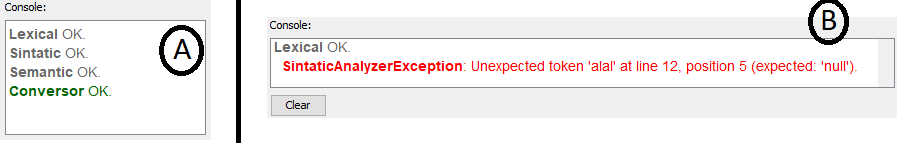
\includegraphics[width=.7\textwidth]{Figuras/tela_compiler_saida.png}
\caption{Saída de dados para na camada view. Lado A mostrando uma compilação com sucesso. Lado B mostrando um erro no Analisador Sintático}
\label{fig:telaCompilerSaida}
\end{figure}

\subsection{Pacote view/util/xmlpack}
Esse pacote contem classes que irão fazer com que a tela "Ontology" e parte da tela "Reasoner" seja um ambiente comum a usuários de arquivos XML, colocando cores e identando de maneira a facilitar a leitura e entendimento do código em XML, como podemos ver nas Figura \ref{fig:telaOntology} e \ref{fig:telaReasoner}. É possível ver o conteúdo do pacote na Figura \ref{fig:pacoteXmlpack}.
\begin{figure}[H]
\centering
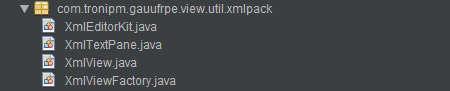
\includegraphics[width=.6\textwidth]{Figuras/pacote_xmlpack.png}
\caption{Classes do pacote .../view/util/xmlpack}
\label{fig:pacoteXmlpack}
\end{figure}

\subsection{Pacote view/util/popupmenu}
As classes desse pacote farão com que, ao usuário pressionar o botão direito, em alguma tela, algumas opções irão aparecer como por exemplo: copiar, colar, recortar, etc. Isso faz com que o usuário se sinta mais confortável e ambientado com o programa, visto que essa é uma prática comum em softwares. Os arquivos desse pacote podem ser visualizados na Figura \ref{fig:pacotePopupmenu}.
\begin{figure}[H]
\centering
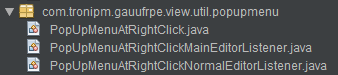
\includegraphics[width=.6\textwidth]{Figuras/pacote_popupmenu.png}
\caption{Classes do pacote .../view/util/popupmenu}
\label{fig:pacotePopupmenu}
\end{figure}

\subsection{Pacote view/util}
Essas classes são as responsáveis por fazer a tela inicial do programa, Compiler, aparentar ser um campo de texto de uma IDE convencional. Colocando número de linhas, mudando cor da linha onde o cursor se encontra, bem como mudando a cor do número na linha onde o cursor se encontra. Também é uma prática muito comum no desenvolvimento de softwares. A Figura \ref{fig:pacoteViewUtil} mostra os arquivos desse pacote.
\begin{figure}[H]
\centering
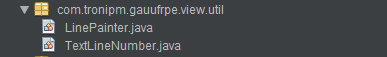
\includegraphics[width=.6\textwidth]{Figuras/pacote_view_util.png}
\caption{Classes do pacote .../view/util}
\label{fig:pacoteViewUtil}
\end{figure}.

\subsection{Pacote view}
Esse pacote é o responsável por armazenar as classes contendo todas as telas propriamente ditas (Figuras \ref{fig:telaCompiler}, \ref{fig:telaOntology}, \ref{fig:telaReasoner} e \ref{fig:telGraph}). Os arquivos que estão dentro do pacote podem ser visto na Figura \ref{fig:pacotesView}.


\section{Model}

Essa camada é responsável por conter classes que denotam o comportamento do sistema, ou seja, a regra de negócio.
\begin{figure}[H]
\centering
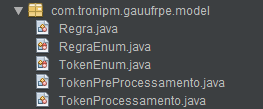
\includegraphics[width=.6\textwidth]{Figuras/pacote_model.png}
\caption{Classes do pacote .../model}
\label{fig:pacotesModel}
\end{figure}

A classe "Regra" é utilizada no processo de análise sintática do compilador. É o equivalente a uma regra de produção no universo de compiladores. A classe "RegraEnum" é apenas definições utilizadas na classe "Regra". A classe "TokenPreProcessamento" é utilizada pelo analisador léxico e sintático, já a classe "TokenProcessamento" é utilizado pelo analisador sintático e semântico, bem como o conversor. As classes de tokens possuem informações como o lexema, coluna, linha, tipo, etc. A classe "TokenEnum" está para "TokenPreProcessamento" assim como a classe "RegraEnum" está para a classe "Regra".

\section{Controller}

Uma vez definido o comportamento dos dados e a interface do usuário, é preciso fazer uma interface entre essas duas camadas. Essa interface em questão é chamada de controller. Ela é responsável por coletar a ação e eventos do usuário, processar e trocar informações com o model. Os controllers podem ser vistos na Figura \ref{fig:pacotesController}.

\begin{figure}[H]
\centering
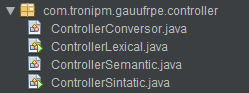
\includegraphics[width=.7\textwidth]{Figuras/pacote_controller.png}
\caption{Classes do pacote .../controller}
\label{fig:pacotesController}
\end{figure}

% -------------------------------------- COMENTADO -----------------------------------
\fi

\subsection{Gramática}

Idiomas como o português, inglês e espanhol possuem um conjunto de regras e normas bem definidas. Isto permite que pessoas com conhecimento destas regras comuniquem-se entre si, tanto no ato de escrever como no de ler. O conjunto dessas regras é chamado gramática. Assim como em um idioma normal, um compilador precisa de regras e normas gramaticais. Isso garante que, ao usuário escrever seu código, ele será entendido por outras pessoas, assim como pelo compilador. Na Tabela \ref{tab:tabelaGramatica} é possível ver a gramática definida para o compilador OrCA IDE. Cada linha é chamada de Regra de Produção. A coluna da esquerda é o título da regra, enquanto a coluna da direita é a regra em si. Para fins de leitura, chamada de regra é feita com <...>, por exemplo <OP>. Chamada de terminal é feita sem <...>, por exemplo \textit{some} ou (. O Símbolo "||" é apenas um separador entre as regras.

\begin{table}[H]
\centering
\caption{Gramática OrCA IDE.}
\label{tab:tabelaGramatica}
\begin{tabular}{|l|l|}
\hline Regra  & Definição  \\ 
\hline <OP>  & \begin{tabular}[l]{@{}l@{}} some || all || only || and || or || isa || equivalent || that \end{tabular} \\
\hline <ID>  & \begin{tabular}[l]{@{}l@{}} a-Z* \end{tabular} \\
\hline <NUM> & \begin{tabular}[l]{@{}l@{}} 0-9* \end{tabular} \\
\hline <FIM> & \begin{tabular}[l]{@{}l@{}} ; || <DEF> || $\varepsilon$ \end{tabular} \\ 
\hline <DEF> & 
\begin{tabular}[l]{@{}l@{}} 
<ID> <OP> <ID> <FIM> \textbf{||} \\
<ID> <OP> (<DEF>) <FIM> || \\
(<DEF>) <OP> <ID> <FIM> || \\
<ID> <OP> <DEF> <FIM> || \\
\end{tabular} \\
\hline
\end{tabular} 
\end{table} 

\subsection{Analisador Léxico}

Este analisador é responsável por fazer o primeiro e menos complexo processamento sobre o código, em linguagem natural, inserido pelo usuário. Esse processamento nada mais é do que receber o texto da interface gráfica e verificar se as palavras e símbolos inseridos pelo usuário são válidos, ou seja, se são aceitos pela gramática do compilador. Essas palavras e símbolos podem ser vistos na Figura \ref{fig:codigoTokenenum}. Com exceção de \textit{END}, \textit{NUMBER} e \textit{IDENTIFIER}, cada palavra e símbolo desta imagem é chamado de "palavra reservada", e não podem ser utilizados para outro fim se não o que foi definido pela gramática deste compilador. O tipo \textit{NUMBER} diz respeito a uma numeração, que pode variar de 1 a ±\textit{n}, ou seja, um número qualquer, já o \textit{IDENTIFIER} diz respeito a uma palavra, que não é reservada pelo compilador, mas foi criada pelo usuário, por exemplo "Cachorro" ou "Vaca". \textit{END} significa que é o final do código inserido pelo usuário. Cada palavra e/ou símbolo inserido pelo usuário é chamado de \textit{token}.

\begin{figure}[H]
\centering
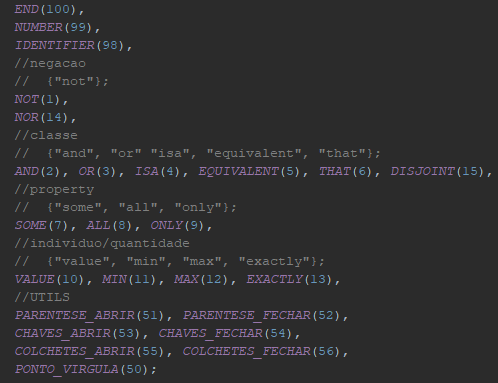
\includegraphics[width=.7\textwidth]{Figuras/codigo_tokenenum.png}
\caption{Palavras reservadas e símbolos permitidos pela gramática}
\label{fig:codigoTokenenum}
\end{figure}

A análise léxica consiste em verificar todos os \textit{tokens}. Caso o \textit{token} não pertença a nenhum dos tipos mostrados na Figura \ref{fig:codigoTokenenum}, irá apresentar uma exceção do tipo \textit{LexicalAnalyzerException}, e o processo de compilação será forçadamente parado (ver Figura \ref{fig:codigoErroLexico}). Caso este \textit{token} pertença a algum dos tipos, ele é adicionado em uma lista de \textit{tokens}. Ao final da análise, essa lista é passada para o Analisador Sintático, encerrando esta análise e mostrando ao usuário que esta etapa foi finalizada com sucesso (ver Figura \ref{fig:codigoSucessoLexico}).

\begin{figure}[H]
\centering
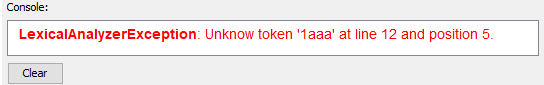
\includegraphics[width=.7\textwidth]{Figuras/codigo_erro_lexico.png}
\caption{Erro do Analisador Léxico sendo mostrado ao usuário na Tela \textit{Compiler}}
\label{fig:codigoErroLexico}
\end{figure}

\begin{figure}[H]
\centering
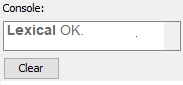
\includegraphics[width=.3\textwidth]{Figuras/codigo_sucesso_lexico.png}
\caption{Analisador Léxico foi executado com sucesso}
\label{fig:codigoSucessoLexico}
\end{figure}

\subsection{Analisador Sintático}

%A arvore de tokens é \textit{top-down}, ou seja, de cima para baixo. Como na gramática não há recursão a esquerda, apenas a direita, a leitura dos \textit{tokens} são feitas da esquerda para direita.

Após a análise léxica, o analisador sintático é acionado. Ele é responsável por identificar se o código inserido pelo usuário faz parte da gramática que o compilador aceita. Em outras palavras, enquanto o analisador léxico se preocupa em verificar se as palavras são aceitas pelo compilador, o analisador sintático verifica se as palavras foram utilizadas na posição correta. Em alguns casos é utilizado \textit{look ahead} de 1 ou 2 tokens para garantir que a leitura na pilha de execução seja a esperada pelo sistema. A Figura \ref{fig:codigoLookAhead} traz um trecho de código do analisador sintático mostrando a utilização de \textit{look ahead}. Esse código verifica se o item atual da pilha é um \textit{not} e, utilizando 1 \textit{token} de \textit{look ahead}, verifica se o próximo item é um \textit{identifier}, e, utilizando mais 1 \textit{token} de \textit{look ahead}, verifica se esse próximo \textit{token} é um operador (\textit{OR}, \textit{AND}, \textit{ISA}, etc).


%for um identificador e lookAhead(2) for "OR, ISA, AND...", então entra no if e adiciona itens a pilha.

\begin{figure}[H]
\centering
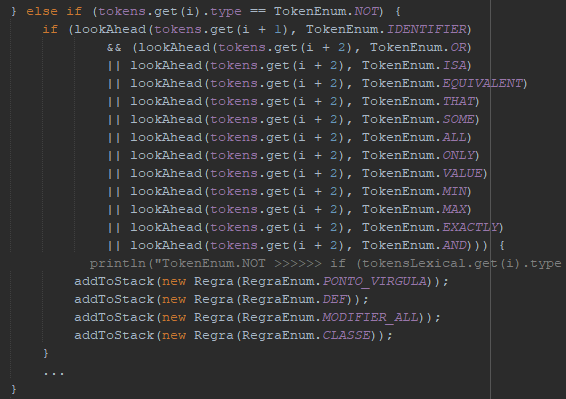
\includegraphics[width=.8\textwidth]{Figuras/codigo_lookahead.png}
\caption{Trecho de código mostrando a utilização do \textit{look ahead}. }
\label{fig:codigoLookAhead}
\end{figure}

Caso alguma expressão do código inserido pelo usuário não pertença a gramática aceita pelo compilador, uma exceção do tipo \textit{SintaticAnalyzerException} será lançada (ver Figura \ref{fig:codigoErroSintatico}). Caso o código do usuário respeite a gramática, esse passo será encerrado, mostrando ao usuário uma mensagem de sucesso (ver Figura \ref{fig:codigoSucessoSintatico}).

%irá passar para o analisador semântico.

\begin{figure}[H]
\centering
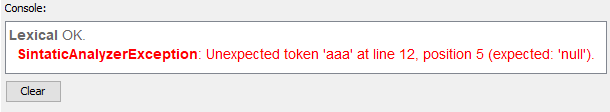
\includegraphics[width=.7\textwidth]{Figuras/codigo_erro_sintatico.png}
\caption{Erro do Analisador Sintático sendo mostrado ao usuário na Tela \textit{Compiler}}
\label{fig:codigoErroSintatico}
\end{figure}

\begin{figure}[H]
\centering
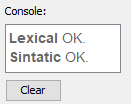
\includegraphics[width=.2\textwidth]{Figuras/codigo_sucesso_sintatico.png}
\caption{Analisador Sintático foi executado com sucesso}
\label{fig:codigoSucessoSintatico}
\end{figure}

\subsection{Analisador Semântico}

Posterior a análise sintática esse controller entra em ação. Ele tem um comportamento diferente dos analisadores semânticos de outros compiladores. A função dele é atomizar o código fonte inserido pelo usuário a fim de criar subexpressões de tamanho mínimo, por exemplo "Homem and Mulher", embora essa expressão faça parte de uma expressão maior denominada "(Homem and Mulher) isa Humano". Essa substituição pode ser vista na Figura \ref{fig:codigoAtomizacao} onde se encontra o código do arquivo ControllerSemantic.java e exibe o momento em que a atomização envolvendo essas palavras reservadas é feita. 

\begin{figure}[H]
\centering
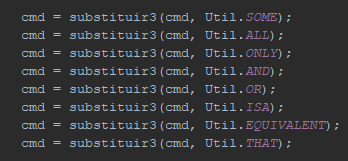
\includegraphics[width=.7\textwidth]{Figuras/codigo_atomizacao.png}.
\caption{Código atomização}
\label{fig:codigoAtomizacao}
\end{figure}

Cada expressão atomizada é inserida em uma lista que será enviada para o ControllerConversor. Caso aconteça algum erro na atomização, uma exceção do tipo SemanticAnalyzerException será lançada (ver Figura \ref{fig:codigoErroSemantico}) na view. Caso o código fonte seja atomizado com sucesso, irá passar para o Controller Conversor.

\begin{figure}[H]
\centering
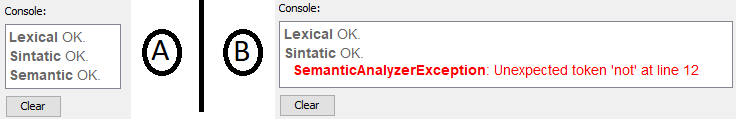
\includegraphics[width=.7\textwidth]{Figuras/codigo_erro_semantico.png}
\caption{Erro Semântico}
\label{fig:codigoErroSemantico}
\end{figure}

A Figura \ref{fig:codigoErroSemantico} está dividida em duas partes, a parte A mostra quando o código passa com sucesso pelo analisador semântico e a parte B mostra quando houve um erro ao tentar atomizar o código fonte


\subsection{Controller Conversor}

Esse \textit{controller} é o responsável por converter o código fonte inserido pelo usuário em uma ontologia. Ao chegar nesse ponto todas as verificações já foram feitas, garantindo que na conversão do código fonte não haja nenhum problema no que diz respeito a parte léxica, semântica e sintática.

\begin{figure}[H]
\centering
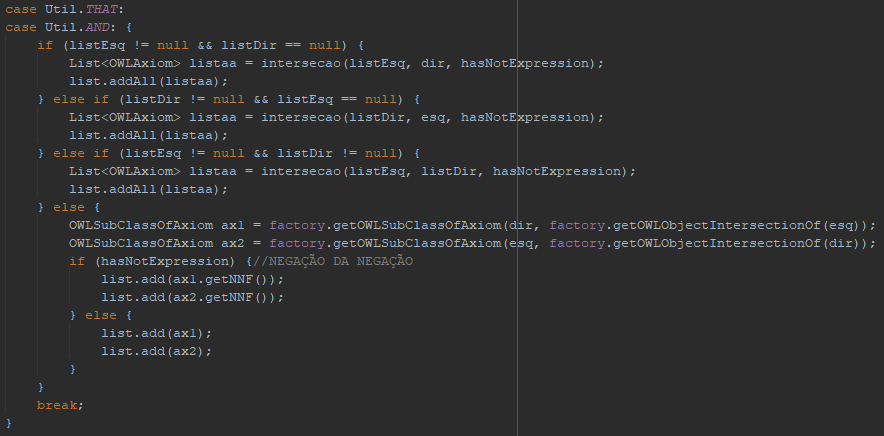
\includegraphics[width=.8\textwidth]{Figuras/codigo_conversor_andthat.png}
\caption{Trecho de código} 
\label{fig:codigoConversor}
\end{figure}

A Figura \ref{fig:codigoConversor} exibe o trecho de código em que ocorre o processo inicial de conversão de expressões AND e THAT, é nessa parte onde é feita a separação quando a expressão é CLASSE vs CLASSE, ou CLASSE vs EXPRESSÃO ou ainda, EXPRESSÃO vs EXPRESSÃO.

\section{Linguagem Natural Controlada}

Para que o usuário consiga utilizar o sistema, será necessário o conhecimento dessa linguagem natural que será definida a seguir, na Tabela \ref{tab:tabelaPalavrasReservadas} se encontra as palavras reservadas, suas respectivas descrições e um exemplo de sua aplicação.

\begin{table}[H]
\centering
\caption{Palavras Reservadas}
\label{tab:tabelaPalavrasReservadas}
\begin{tabular}{|l|l|l|}
\hline Reservado  & Descrição & Exemplo  \\ 
\hline isa & \begin{tabular}[l]{@{}l@{}} Uma classe X é um \\tipo de classe Y.\end{tabular} & Gato isa Felino \\ \hline
equivalent & \begin{tabular}[l]{@{}l@{}} Uma classe X é um tipo \\ de classe irmã de Y.\end{tabular} & JanelaBanheiro equivalent JanelaCasa \\ \hline and / that & \begin{tabular}[l]{@{}l@{}} Uma classe X interseção\\ com uma classe Y.\end{tabular} & (Correr and Pular) isa ExercicioFisico  \\ \hline or & \begin{tabular}[l]{@{}l@{}}Uma classe X disjunção\\ de uma classe Y. \end{tabular} & Trabalhar isa nor(Dormir or Comer) \\ \hline only & \begin{tabular}[l]{@{}l@{}}Uma propriedade X\\ only classe Y. \end{tabular} & podeLatir only Cachorro \\ \hline some & \begin{tabular}[l]{@{}l@{}}Uma propriedade X\\ some classe Y. \end{tabular} & andarNoMuro some Gato \\ \hline all & \begin{tabular}[l]{@{}l@{}}Uma propriedade X \\ all classe Y. \end{tabular} & comerGrama all Vaca \\ \hline not & Negação de uma Classe & not Gato \\ \hline nor & Negação de uma expressão & nor(Gato isa Felino) \\ \hline 
\end{tabular}
\end{table}

Como visto de maneira resumida na Tabela \ref{tab:tabelaPalavrasReservadas}, na Figura \ref{fig:codigoFonteInicial} está o código fonte que o sistema mostra ao ser aberto, para que o usuário entenda o funcionamento da sintaxe.

\begin{figure}[H]
\centering
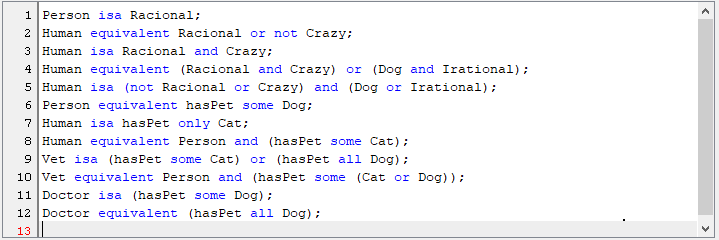
\includegraphics[width=.8\textwidth]{Figuras/codigo_codigofonte_inicial.png}
\caption{Código inicial}
\label{fig:codigoFonteInicial}
\end{figure}

\subsection{Funcionalidades}
NÃO SEI O QUE PODERIA COLOCAR AQUI

Aqui vc vai mostrar as funcionalidades do sistema, inclusive colocar diagramas de casos de uso em UML mostrando quais as funcionalidades os usuários realizam.operando a ferramenta.

\subsection{Conclusões}
Conclusões

Concluir o capítulo, pode deixar sem fazer que eu ajudo. No final da revisão q eu fizer eh melhor pra concluir.


\chapter{Experimentos e Resultados}
\label{chap:conclusao}

TEXTO

\bibliographystyle{estilo_ABNT}
\bibliography{refs}
\addcontentsline{toc}{chapter}{Bibliografia}

\end{document}

 %camadas? Apresentar os módulos existentes. Colocar uma imagem do diagrama de componentes em UML com os módulos existententes.

%(Cada subseção corresponde individualmente a cada módulo da arquitetura do sistema, vc vai falar de cada módulo e de cada componente e sub componente que tem no módulo. Colocar imagens dos submódulos pra n precisar ir na Figura da Seção Arquitetura.

%Vai exemplificar o que ocorre em cada módulo, qual a entrada e o que gera de saída para o próximo módulo.